\documentclass[tikz,border=10pt]{standalone}
\usetikzlibrary{calc,patterns,angles,quotes}
\begin{document}
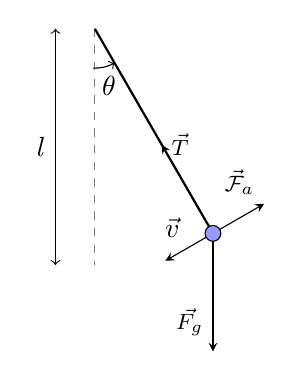
\begin{tikzpicture}
    \pgfmathsetmacro{\Gvec}{1.5}
    \pgfmathsetmacro{\myAngle}{30}
    \pgfmathsetmacro{\Gcos}{\Gvec*cos(\myAngle)}
    \pgfmathsetmacro{\Gsin}{\Gvec*sin(\myAngle)}

    \coordinate (centro) at (0,0);
    \draw[dashed,gray,-] (centro) -- ++ (0,-3.) node (mary) [black,left]{$ $};
    \draw[thick] (centro) -- ++(270+\myAngle:3) coordinate (bob) node[midway,above right] {};
    \pic [draw, ->, "$\theta$", angle eccentricity=1.5] {angle = mary--centro--bob};
    \draw [black,-stealth] (bob) -- ($(bob)!\Gcos cm!(centro)$)
    	node[right] {\footnotesize{$\vec{T}$}} ;
    \draw [-stealth] (bob) -- ($(bob)! -\Gsin  cm!90:(centro)$)
      coordinate (gsin)
      node[above left] {\footnotesize{$\vec{{\mathcal{F}}}_{a}$}};
    \draw [-stealth] (bob) -- ($(bob)! -1.5 +\Gsin cm!90:(centro)$)
      coordinate (gsin)
      node[midway,above left] {$\vec{v}$};
 	 \draw[-stealth,<->] (-0.5,0) -- (-0.5,-3.)  node[midway, left] {$l$};
    \draw [-stealth] (bob) -- ++(0,-\Gvec)
      coordinate (g)
      node[near end,left] {\footnotesize{$\vec{{F_{g}}}$}};
   
    \filldraw [fill=blue!40,draw=black] (bob) circle[radius=0.1];
    
  
\end{tikzpicture}
\end{document}